% !TeX encoding = UTF-8
\documentclass[12pt]{article}
\usepackage[utf8]{inputenc}
\usepackage[T2A]{fontenc}
\usepackage[russian]{babel}
\usepackage{graphicx}
\usepackage{listings}
\usepackage{xcolor} 
\usepackage{indentfirst}
\usepackage{textcomp}
\usepackage{tempora}
\usepackage{indentfirst}
\usepackage{amsmath,amsfonts,amssymb,amsthm,mathtools} % AMS
\usepackage{icomma}
\usepackage{mathrsfs}
\usepackage{fancyhdr}
\usepackage{hyperref}
\definecolor{medium-blue}{rgb}{0,0,1}
\hypersetup{colorlinks, urlcolor={medium-blue}}
\lstset{  
	basicstyle=\fontsize{11}{13}\scriptsize\ttfamily,
	commentstyle=\ttfamily\color{gray},
	numbers=left,
	numberstyle=\ttfamily\color{gray}\footnotesize,
	stepnumber=1,
	numbersep=10pt,
	backgroundcolor=\color{gray!10},
	rulecolor=\color{black!30},
	showspaces=false,
	showstringspaces=false,
	showtabs=false,
	frame=single,
	tabsize=2,
	captionpos=b,
	breaklines=true,
	breakatwhitespace=false,
	title=\lstname,
	 escapeinside={(*}{*)},
	keywordstyle={},
	morekeywords={},
	extendedchars=true,
	inputencoding=utf8
}

\begin{document}

\begin{titlepage}

\newcommand{\HRule}{\rule{\linewidth}{0.5mm}} 
\centering 
%----------------------------------------------------------------------------------------
%	HEADER
%----------------------------------------------------------------------------------------
\textsc{\LARGE Параллельное и распределённое программирование }\\[0.5cm] 
\textsc{\Large Отчет }\\[0.5cm] 
%----------------------------------------------------------------------------------------
%	TITLE
%----------------------------------------------------------------------------------------
\HRule \\[0.4cm]
{ \huge \bfseries Лабораторная работа № 2}\\[0.4cm]
\HRule \\[1.5cm]

%----------------------------------------------------------------------------------------
%	AUTHOR
%----------------------------------------------------------------------------------------
\begin{minipage}{0.4\textwidth}
\begin{flushleft} \large
\emph{Автор:}\\
Поташев Н. А.\\
\end{flushleft}
\end{minipage}
~
\begin{minipage}{0.4\textwidth}
\begin{flushright} \large
\emph{Руководитель:} \\
Рудалев А. В.
\end{flushright}
\end{minipage}\\[2cm]

%----------------------------------------------------------------------------------------
%	DATE
%----------------------------------------------------------------------------------------
{\large \today}\\[2cm] 
%----------------------------------------------------------------------------------------
%	LOGO
%----------------------------------------------------------------------------------------
\includegraphics[scale=0.2]{logo.pdf} 
%----------------------------------------------------------------------------------------
\vfill
\end{titlepage}


\section{Постановка задачи}
Целью данной лабораторной работы было сравнение параллельной и последовательной реализации алгоритма решения краевой задачи Дирихле для уравнения Пуассона.
	\[
	\begin{cases}
	\frac{\partial^2u}{\partial x^2} + \frac{\partial^2u}{\partial y^2} = f(x,y)  ,\quad(x,y)\in D\\
	u(x,y)=g(x,y) ,\quad(x,y)\in D^{0}
	\end{cases}
	\]
В качестве области задания D функции u(x,y) был использован единичный квадрат 
\[D=\{(x,y)\in D: 0 \leq x \leq 1\}.\]
Во время выполнения работы был рассмотрен следующий пример задачи Дирихле:
найти стационарное распределение температуры в квадратной пластине со стороной 1, описываемое уравнением Лапласа(частный случай, когда f(x,y)=0)
с краевыми условиями вида:
	\[
	\begin{cases}
	f(x,y)=0, \quad(x,y)\in D,\\
	0 , \qquad \text{ if}  \quad x=0, \\
	sin(y) ,\text{ if}\quad x=1, \\
	0 , \qquad \text{ if}\quad y=0, \\
	sin(x) ,\text{ if}\quad y=1. \\
	\end{cases}
	\]
Список вариантов для решения задачи Дирихле(вариант 15).\footnote{\url{http://old.exponenta.ru/educat/systemat/hanova/lab/LR7/LR7.asp}.}
\section{Выполнение работы}
В ходе выполнения данной работы были получены:
	\begin{itemize}
		\item программа, реализующая параллельное и последовательное решения задачи Дирихле;
		\item python-скрипт, реализующий построение графиков на основе полученных данных;
		\item bash-скрипт для запуска программы на ПК;
		\item sbatch-скрипт для запуска программы на кластере;
		\item результаты расчетов программы на кластере и ПК(в формате csv-файлов).
	\end{itemize}

\subsection{Алгоритмы}
Был реализован сначала последовательный алгоритм решения задачи Дирихле методом сеток, а после были приняты попытки реализовать параллельную версию алгоритма см. Листинг 1-4.
	\begin{lstlisting}[language=c++,caption=реализация последовательного алгоритма,label=first:linear]
	...	
double max;
do {
	max = 0;
	for (size_t i = 1; i < size + 1; ++i)
		for (size_t j = 1; j < size + 1; ++j) {
			double u0 = u(i, j);
			double temp = 0.25 * (u(i-1, j) + u(i+1, j) + u(i, j-1) + u(i, j+1) - h*h*F(i - 1, j - 1));
			u(i, j) = temp;
			double d = std::fabs(temp - u0);
			
			if (d > max) {
			max = d;
		}
	}
} while (max > eps);
	...
	\end{lstlisting}
Для представления u был выбран ранее реализованный класс Matrix.	
	\begin{lstlisting}[language=c++,caption=неудачная реализация параллельного алгоритма(пример data race),label=first:para]	
	...
double max;
do {
	max = 0;
	#pragma omp parallel for shared(u)  //worst
	for (size_t i = 1; i < size + 1; ++i)
		for (size_t j = 1; j < size + 1; ++j) {
			double u0 = u(i, j);
			double temp = 0.25 * (u(i-1, j) + u(i+1, j) + u(i, j-1) + u(i, j+1) - h*h*F(i - 1, j - 1));
			u(i, j) = temp;
			double d = std::fabs(temp - u0);
			
			if (d > max) {
			max = d;
		}
	}
} while (max > eps);
	...
	\end{lstlisting}
\newpage
	\begin{lstlisting}[language=c++,caption=реализация медленного параллельного алгоритма,label=second:para]	
	...
omp_lock_t lock;
omp_init_lock(&lock);

do {

	max = 0;
	#pragma omp parallel for shared(u,size,max) private(i,j,temp,d,dm) 
	for (i = 1; i < size + 1; ++i)
	{	
		dm = 0;
		for (j = 1; j < size + 1; ++j) {
		
			temp = u(i, j);
			un(i,j) = 0.25 * (u(i-1, j) + u(i+1, j) + u(i, j-1) + u(i, j+1) - h*h*F(i-1, j-1));
			d = std::fabs(temp - un(i,j));
		
			if (dm < d) {
				dm = d;
			}
		
			omp_set_lock(&lock);
			if ( max < dm ) {
				max = dm;
			}
			omp_unset_lock(&lock);
			}
	}
	for (i = 1; i < size + 1; ++i){	
	
		for (j = 1; j < size + 1; ++j) {
	
		u(i,j)=un(i,j);
	
		}
	}
	
} while (max > eps);
	...
	\end{lstlisting}
Данный алгоритм обладал плохой сходимостью и был очень медленным. Поэтому было решено игнорировать эту реализацию.	
	\begin{lstlisting}[language=c++,caption=реализация параллельного алгоритма,label=third:para]	
	...
std::vector<double> mx(size+1);
do
{
	
		for (size_t k = 1; k < size+1; k++) {
			mx[k] = 0;
			#pragma omp parallel for shared(u_mat,k,mx) private(i,j,u0,d)
			for (i = 1; i < k+1; i++) {
				j = k + 1 - i;
				u0 = u_mat(i, j);
				u_mat(i, j) = 0.25 * (u_mat(i-1, j) +u_mat(i+1, j) + u_mat(i, j-1) + u_mat(i, j+1) - h*h*f_mat(i-1, j-1));
				d = std::fabs(u_mat(i, j) - u0);
				if (d > mx[i]) mx[i] = d;
			}
		}
		for (size_t k = size-1; k > 0; k--) {
		#pragma omp parallel for shared(u_mat,k,mx) private(i,j,u0,d)
			for (i= size-k+1; i < size+1; i++){
				j = 2*size - k - i + 1;
				u0 = u_mat(i, j);
				u_mat(i, j) = 0.25 * (u_mat(i-1, j) +u_mat(i+1, j) + u_mat(i, j-1) + u_mat(i, j+1) - h*h*f_mat(i-1, j-1));
				d = std::fabs(u_mat(i, j) - u0);
				if (d > mx[i]) mx[i] = d;				
		}
	}
	max = 0;
	for (size_t i = 1; i < size+1; i++) {
		if (mx[i] > max) max = mx[i];
	}
} while (max > eps);
	...
	\end{lstlisting}
Именно этот алгоритм был выбран для решения задачи, так как он обладал такой же сходимостью, что и последовательный вариант, при этом был более эффективным за счет параллельных участков кода.
\subsection{Результаты расчетов}
Результатом выполнения программы был текстовой csv-файл c полученной поверхностью и временем работы программы. Были выполнены расчеты на ПК и кластере, также был нарисован график поверхности см Рис. 1, графики эффективности, времени работы, ускорения программы при параллельной реализации см Рис. 2-3.
\\
	\begin{figure}
		\centering
		\includegraphics[scale=0.7]{pc/surface4.pdf}
		\caption{результат работы программы - поверхность}
		
		\includegraphics[scale=0.7]{pc/eff_plots.pdf}
		\caption{графики эффективности работы на ПК}
	\end{figure}
\newpage
	\begin{figure}
		\centering
		\includegraphics[scale=0.7]{cluster/eff_plots.pdf}
		\caption{графики эффективности работы на кластере}
	\end{figure}
	
\newpage
\section{Вывод}
По рис. 2-3 можно сделать вывод, что параллельный алгоритм решения задачи Дирихле более эффективный, чем последовательный. Реализованный волновой алгоритм не является самым оптимальным, так как не полностью использует поистине огромный потенциал кэша процессора. Проблемным местом алгоритма является то, что мы итеративно просчитываем диагонали матрицы, и расчет первого элемента \[u_{1,1}\] нельзя распараллелить, так как он один. В будущем можно модифицировать алгоритм следующими способами: 
	\begin{itemize}
		\item блочное разделение диагоналей;
		\item использование очереди;
		\item расчет диагоналей матрицы от концов к середине(или наоборот).
	\end{itemize}
\end{document}